\lsection{Design}{design}
\subsection{Ceremony Protocol}

Here we describe a MPC protocol for $N$ contributors $C_1, \ldots C_N$ to participate in the computation of the public parameters $\sigma$. Because the participants must contribute in serial, we use a central \Coordinator{} to order the participants and check their contributions. We emphasize that the \Coordinator{} exists solely to help organize the ceremony and has no effect on the security properties of the MPC.

The protocol is initialized by the \Coordinator{} and proceeds in repeated rounds, in which the \Coordinator{} and a \Contributor{} exchange messages. The messaging protocol is described in Section \ref{sec: MessagingProtocol}.

\subsubsection*{Initialization}

The \Coordinator{} computes an initial state $\sigma_0$ and challenge hash $c_0$ as 
\begin{equation*}
    (\sigma_0, c_0) =  \initialize{}(\text{circuits, KZG parameters})
\end{equation*} 
The inputs to \initialize{} are the QAP descriptions \eqref{eqn: qap} of some ZK circuits and modified KZG parameters \eqref{eq: kzg} (the output of a prior Phase 1 ceremony). The function \initialize{} computes $\sigma_0$, a Groth16 proving key with $\delta = 1$ (see \eqref{eq: prover_key}), and an initial challenge hash $c_0$.

Note that \initialize{} is deterministic and the circuit descriptions and KZG parameters are public. Therefore any observer may verify that \Coordinator{} completed this step correctly.

\subsubsection*{Contribution Round}

The $n^{\text{th}}$ round of contribution begins with the state $\sigma_{n-1}$ and challenge $c_{n-1}$ of the previous round. \Contributor{} $C_n$ will interact with \Coordinator{} to produce the next state $\sigma_{n}$ and a proof $\pi_{n}$ that it was computed according to the protocol. The round consists of these steps: (refer to Section \ref{sec:phase2})

\begin{enumerate}
\item \Coordinator{} sends $(\sigma_{n-1}, c_{n-1})$ to \Contributor{} $C_n$.
\item \Contributor{} computes $(\sigma_n, \pi_n) = $ \contribute{}$(\sigma_{n-1}, c_{n-1})$.
\item \Contributor{} sends $(\sigma_n, \pi_n)$ to \Coordinator{} (as a signed message)
\item \Coordinator{} computes \verify{}$(\sigma_{n-1}, c_{n-1}, \sigma_n, \pi_n)$. This checks that the \Contributor{} has formed $\sigma_n$ from $\sigma_{n-1}$ according to the protocol.
    \begin{enumerate}
        \item If the check fails, \Coordinator{} rejects this contribution. Nothing is added to the transcript and the \Coordinator{} proceeds to next round with state and challenge unchanged ($\sigma_n = \sigma_{n-1}$ and $c_n = c_{n-1}$).
        \item Otherwise, \Coordinator{} computes challenge $c_n = $ \challenge$(\sigma_{n-1}, c_{n-1}, \sigma_n, \pi_n)$ and records $\sigma_n, \pi_n, c_n$ to the \Transcript{}.
    \end{enumerate}
\item \Coordinator{} proceeds to next round with $(\sigma_n, c_n)$.
\end{enumerate}
This process repeats until all \Contributor{}s have made their contribution. At the end (assuming all contributions were valid) we have a Groth16 prover key $\sigma$ with $\delta = \delta_1 \cdot \delta_2 \cdot \ldots \cdot \delta_N $ and a \Transcript{} $T = \{ (\sigma_i, \pi_i, c_i) \}_{i=1}^N $ recording all contributions to the ceremony and allowing a third-party to verify that $\sigma$ was computed according to protocol.

\subsection{Messaging Protocol}\label{sec: MessagingProtocol}

In each round, the \Coordinator{} and \Contributor{} communicate via (unencrypted?) messages. Messages from the \Contributor{} to the \Coordinator{} are signed with an Ed25519 signature. The \Coordinator{} accepts only those messages with a valid signature whose public verifying key belongs to a \Registry{} of participants. The \Registry{} and signature checks prevent a DDoS attack on the ceremony in which malicious participants fill up the contribution queue and intentionally time-out without contributing.

The \Contributor{} sends one of two messages to the \Coordinator{}: a \QueryRequest{} or an \UpdateRequest{}. Each message follows the format 
\begin{center} 
    (Participant ID | Domain Tag | Nonce | Payload). 
\end{center}
In a \QueryRequest{} the Payload is empty, whereas in an \UpdateRequest{} the Payload contains a new state and proof, $(\sigma_n, \pi_n)$. In both cases the message is serialized to bytes and signed with an Ed25519 signature.

The \Coordinator{} responds to these messages according to the current state of the protocol:
\begin{itemize}
    \item \QueryRequest{}: the \Coordinator{} responds with a \QueryResponse{} containing:
        \begin{itemize}
            \item Current state $\sigma_{n-1}$ and challenge $c_{n-1}$, if \Contributor{} is at front of \Queue{} (see below).
            \item \Contributor{}'s current position in \Queue{}, if \Contributor{} is not at front of queue.
            \item Error messsage, if \Contributor{} has already participated in ceremony.
        \end{itemize}
    \item \UpdateRequest{}: the \Coordinator{} responds with an \UpdateResponse{} informing the \Contributor{} of whether their contribution was successfully verified.
    \item If the message from \Contributor{} fails signature verification, the \Coordinator{} responds with the expected nonce for the \Contributor{}'s Participant ID. (If the Participant ID is invalid the \Coordinator{} ignores the message.)
\end{itemize}

\subsection{Server State Machine}

The \Coordinator{} role is performed by a central server state machine. The \Coordinator{}'s duties are to enforce the MPC protocol and organize the contributions. 

To enforce the MPC protocol, the \Coordinator{} performs:
\begin{itemize}
    \item Parameter Initialization: a reproducible initial state $\sigma_0$ and initial challenge $c_0$ are computed from public data.
    \item Contribution Verification: each contribution to the ceremony is checked to conform to the MPC protocol.
    \item Contribution Archival: each successful contribution to the ceremony is recorded, together with the proof that it conforms to the MPC protocol.
\end{itemize}
To organize the contributions, the \Coordinator{} performs:
\begin{itemize}
    \item Registry Maintenance: a registry of authorized participants is kept.
    \item Signature Verification: all messages from a \Contributor{} to the \Coordinator{} will be signed.
    \item Queue Management: during the ceremony, participants are ordered in a queue.
\end{itemize}

\subsubsection*{State}
The above \Coordinator{} tasks are accomplished by a machine whose state consists of:
\begin{itemize}
    \item \Registry{}: For each participant, a record of their public signing key, current signature nonce, and whether they have already contributed to the ceremony.
    \item \MpcState{}: The current pair $(\sigma_n, c_n)$ (see Section \ref{sec:phase2}). 
    \item \Transcript{}: The history of MPC states and proofs.
    \item \Queue{}: an ordering of the participants waiting to contribute. This may be a priority queue, if desired.\footnote{A priority queue can help defend against a DDoS attack in which malicious participants intentionally time out without contributing. If a participant times out too many times they can be de-prioritized, allowing more reliable participants to skip them in the queue.}
    \item \TimedLock{}: a lock is given to the participant at the front of the queue while they compute their contribution. This lock times out after a specified duration and drops the participant from the queue.
\end{itemize}

\subsubsection*{State Changes}
The following function calls change the state of the machine:
\begin{itemize}
    \item \initialize{}: set \MpcState{} to $(\sigma_0, c_0)$ (see above).
    \item \enqueue{}(\ParticipantId{}): check that participant is registered and has not already contributed. If so, add to end of \Queue{}.
    \item \textsf{register}: add new participants to the \Registry{}.
    \item \update{}: Compute \verify{}$(\sigma_{n-1}, c_{n-1}, \sigma_n, \pi_n)$ to check that the latest contribution conforms to MPC protocol. If so, 
        \begin{itemize}
            \item compute challenge $c_n$, update \MpcState{} to $(\sigma_n, c_n)$
            \item Add $(\sigma_n, \pi_n, c_n)$ to \Transcript{}
            \item Set participant's contribution status in \Registry. 
            \item Update \Queue{} and \TimedLock{}.
        \end{itemize}
        If contribution is invalid, update only \Queue{} and \TimedLock{} (and downgrade participant's \Queue{} priority, if applicable).
\end{itemize}

\subsubsection*{Operation}
The \Coordinator{} state machine initializes its state and then listens for messages and processes these according to the messaging protocol (see above). Two types of messages are recognized, \QueryRequest{} and \UpdateRequest{}. The state machine responds in the following way to each request:
\begin{itemize}
    \item \QueryRequest{}
    \begin{enumerate}
        \item Parse \ParticipantId{} from request. 
        \item Consult \Registry{}, confirm participant is registered and has not contributed. 
        \item Consult \Queue{}; if participant is not in \Queue{}, call \enqueue{}.
        \item Consult \Queue{}; if participant is at front of \Queue{}, send a message containing \MpcState{} to participant and set \TimedLock{}. Otherwise, send participant a message containing their current position in \Queue{}.
    \end{enumerate}
    \item \UpdateRequest{}
    \begin{enumerate}
        \item Parse \ParticipantId{} from request. Check that the \TimedLock{} refers to this participant.
        \item Parse state, proof $(\sigma_n, \pi_n)$ from request. 
        \item Call \update{}$(\sigma_{n-1}, c_{n-1}, \sigma_n, \pi_n)$.
    \end{enumerate}
\end{itemize}
If any of the above checks do not pass, the \Coordinator{} responds with an appropriate error message.

The operation of this machine is summarized in Figure \ref{fig: server}.

\subsection{Client State Machine}

The duty of a \Contributor{} is to contribute according to the MPC protocol. To this end, a client state machine performs:
\begin{itemize}
    \item Ed25519 Keypair Generation: each \Contributor{} generates their own signature credentials.
    \item Message Signing: messages to \Coordinator{} are signed.
    \item Contribution: formed according to MPC protocol.
\end{itemize}

\subsubsection*{State}
The state of this machine is an Ed25519 private key and a message nonce (unsigned integer). The only state changes during operation are updates to the message nonce. The machine also needs access to some random oracle to perform keypair generation and contribution.

This state is initialized by \generatekeypair{}, which generates an Ed25519 private/public keypair. Note that the same state can later be recovered by prompting users to enter their private key or seed phrase (the correct nonce can be recovered by queries to the server).

\subsubsection*{Operation}

\begin{enumerate}
    \item Initialize state.
    \item Send signed \QueryRequest{} to \Coordinator{}. Await response containing \MpcState{} and challenge, $(\sigma_{n-1}, c_{n-1})$.
    \item Compute $(\sigma_n, \pi_n) = $ \contribute{}$(\sigma_{n-1}, c_{n-1})$.
    \begin{enumerate}
        \item Sample random $\delta$
        \item Transform $\sigma_{n-1}$ by $\delta$ to get $\sigma_n$
        \item Produce ratio proof $\pi_n$ 
    \end{enumerate}
    \item Send signed \UpdateRequest{} to \Coordinator{}. Await response confirming submission.
    \item Clear $\delta$ from memory.
\end{enumerate}

\begin{figure}
    \caption{Operation of the server state machine.}\label{fig: server}
    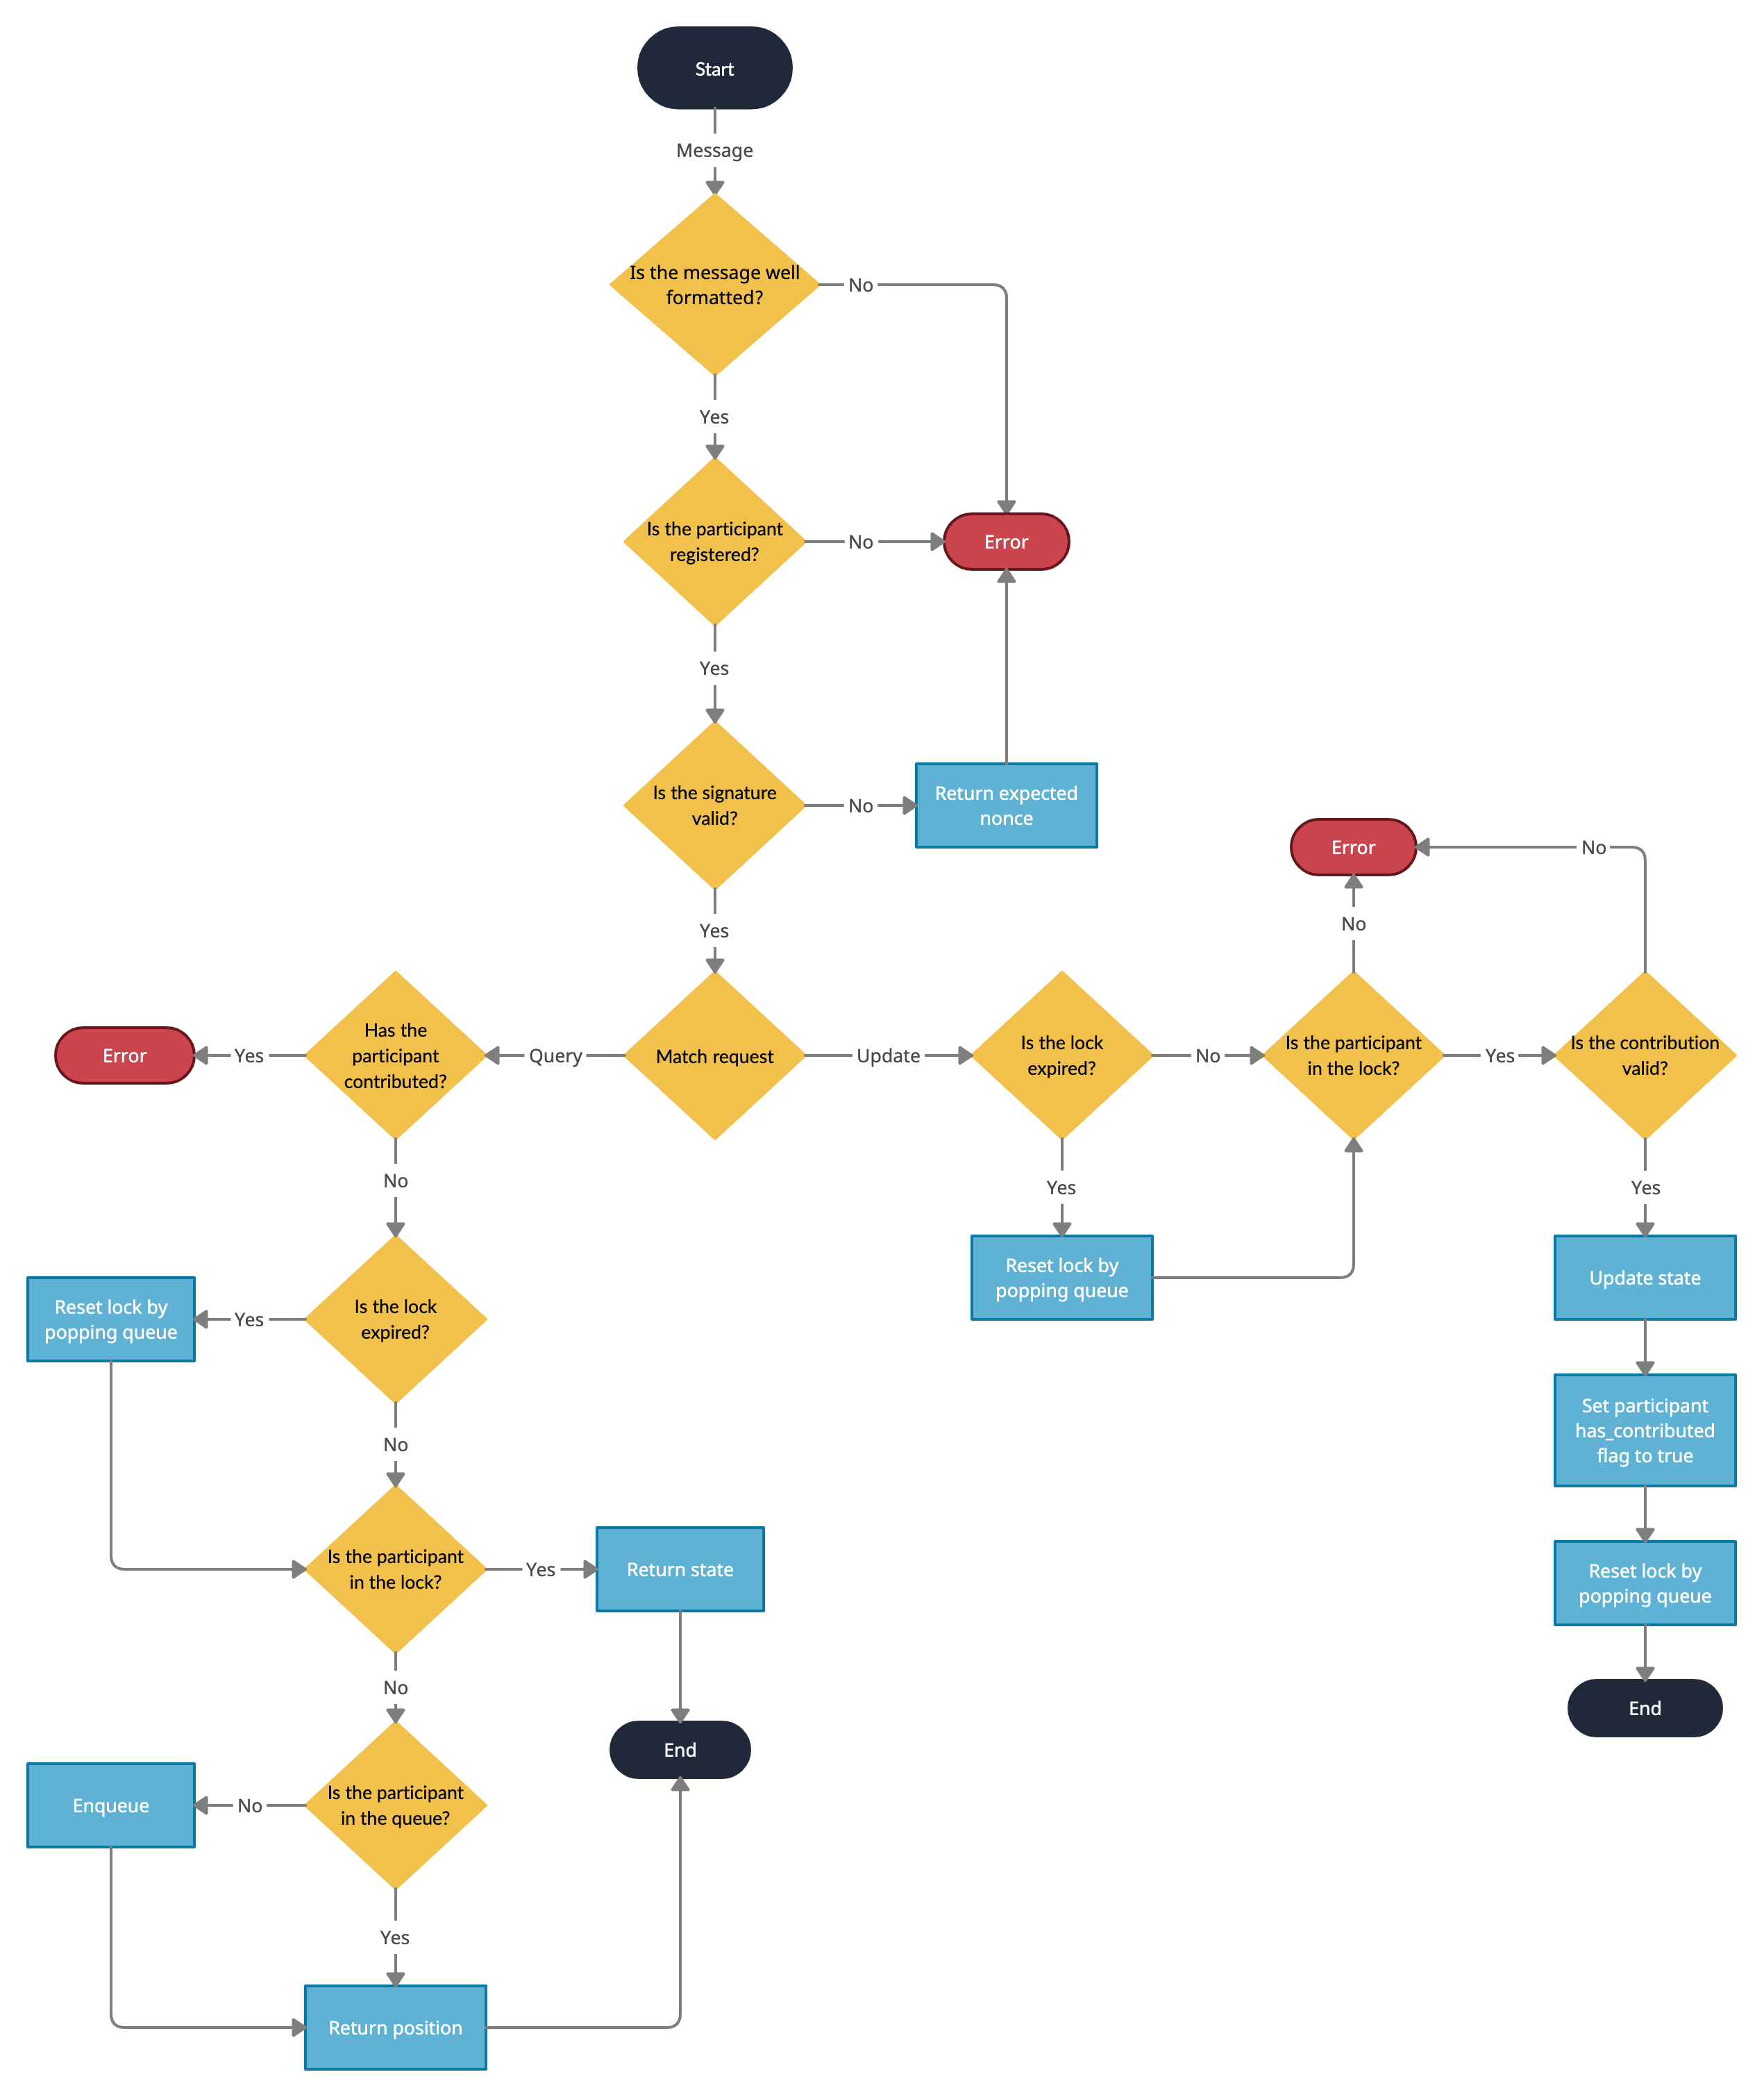
\includegraphics[width = \textwidth]{diagrams/server-state-machine.png}
\end{figure}
    